
\section{Autoren}

Durch die im Abschnitt \ref{communities} gefundenen Communities kann man jetzt auch die Beziehung 
eines Autors zu der ihm zugeordneten Community betrachten. \\

In diesem Abschnitt wird untersucht ob verschiedene Rollenverteilungen unter den Autoren einer Community erkennbar sind.
Hierbei wird festgestellt welche Rollen unter den Autoren auftreten und welche Rolle etwa, die Autoren einnehmen die am 
meisten publizieren. \\

Dazu wurden die in \cite{hubsconnectors} beschriebene Klassifizierung von Knoten verwendet. Um die Knoten klassifizieren zu k�nnen 
muss jeweils die With-in-module-degree (z-score) und
f�r sie und ihre Communities berechnet werden. 
\begin{center}
					\hpic{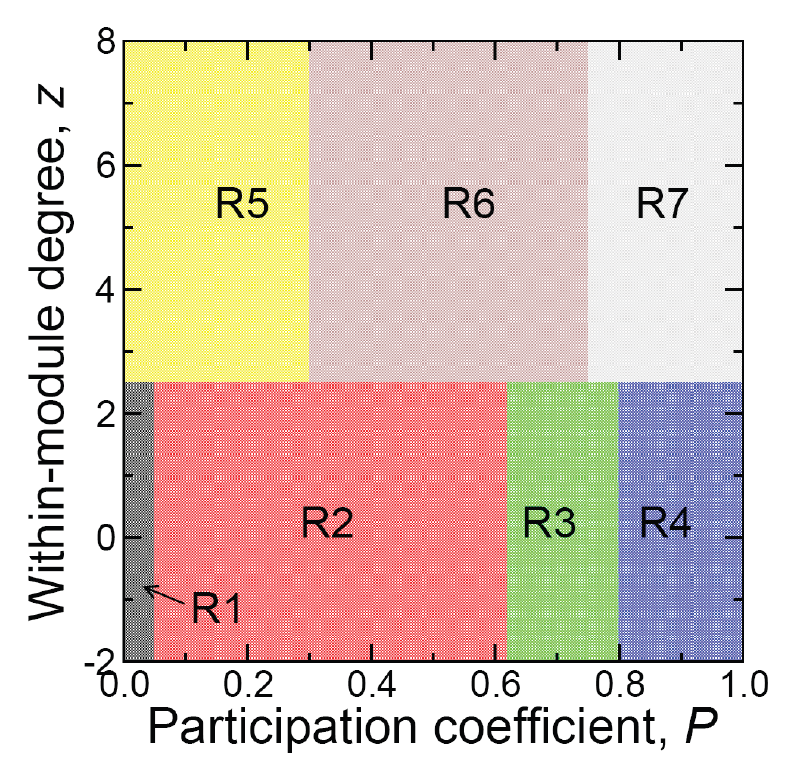
\includegraphics[width=0.7\textwidth]{images/r1_r7.png}
					} \newcaption{Klassifizierung der Author-Knoten}
					\label{fig:r1_r7}
\end{center}
Anschlie�end 
kann die Klassifizierung des Knotens wie in Abbildung \ref{fig:r1_r7} beschrieben erfolgen. Grunds�tzlich wird in diesem Model 
zwischen folgenden Rollen unterschieden:

\begin{itemize}

\item Nabenknoten (hubs) 

\begin{description}
 \item [(R5) provincial hubs] (provinzielle Naben/Zentren)
 \item [(R6) connector hubs] (verbindende Naben/Zentren)
 \item [(R7) kinless hubs] (sippenlose Naben/Zentren)
\end{description}

 \item Einzelknoten (non-hubs) 
\begin{description}
 \item [(R1) ultraperipheral] (sehr dezentral)
 \item [(R2) peripheral] (dezentral)
 \item [(R3) connectors] (Bindeglieder)
 \item [(R4) kinless vertices] (Einzelknoten)
\end{description}

\end{itemize}

Zur Klassifizierung der Autor-Knoten im Co-Autor-Graphen, wird f�r jeden Knoten die Community betrachtet in der er sich befindet (Top-Level-Community). 


% {Teilfrage: Sind verschieden Rollenverteilungen unter den Autoren einer Community erkennbar ?}
% { Methoden }

% { Ergebnisse }
\begin{center}
					\hpic{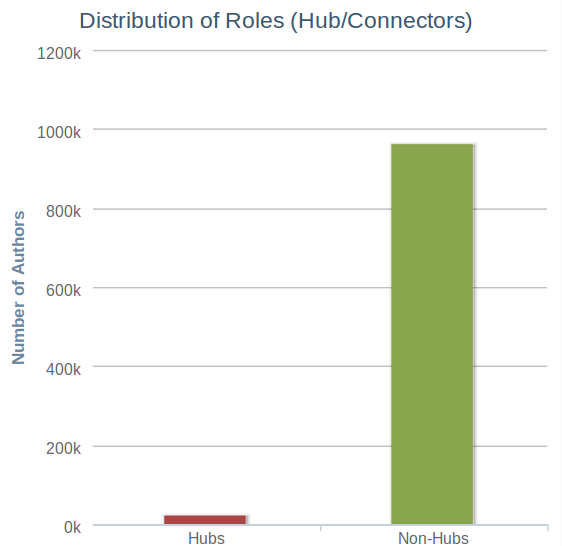
\includegraphics[width=0.7\textwidth]{final_results/roles_hub_con.png}
					} \newcaption{Verteilung der Rollen}
					\label{fig:r1_r7}
\end{center}

\begin{center}
					\hpic{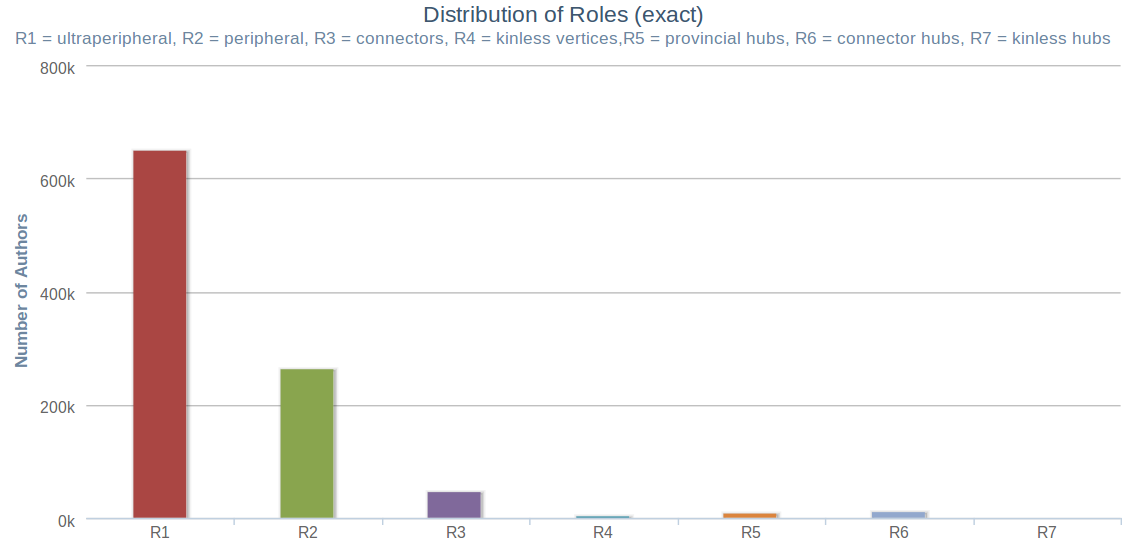
\includegraphics[width=0.7\textwidth]{final_results/roles_r1r7.png}
					} \newcaption{Verteilung der Rollen}
					\label{fig:r1_r7}
\end{center}
% { Diskussion }